\documentclass[paper=a4,11pt,titlepage,twoside=true,headings=normal,numbers=noenddot,captions=tableabove,listof=totoc,index=totoc,bibliography=totoc]{scrreprt}
%\usepackage{amsmath} % abgesetzte Formeln zentriert in der Zeile
%\usepackage[fleqn,intlimits]{amsmath} % [fleqn] abgesetzte Formeln mit festem Abstand zum linken Rand
\usepackage[reqno,intlimits]{amsmath} % [reqno] um die gleichungsnummerierung rechts zu haben
% intlimits: Grenzen für Integrale unterhalb und oberhalb des Zeichens
\usepackage{amssymb}
\usepackage{array}
%\usepackage[ngerman]{babel}
%\usepackage[ngerman]{varioref}
\usepackage[english]{babel}
\usepackage[english]{varioref}
\usepackage[T1]{fontenc} 
\usepackage[utf8]{inputenc}
%---------------------------
\usepackage{booktabs}
\usepackage{calc}
\usepackage{cancel}
\usepackage[labelfont={footnotesize,sf,bf},textfont={footnotesize,sf}]{caption} %Format (Textgröße, Textform) für Bildtext 
%normalsize
%scriptsize
% sc --> smallcaps
% bf --> bold face
% sf --> sans serif
%\usepackage{cite} %inkompatibel mit biblatex
\usepackage[table]{xcolor}
%\usepackage{colortbl}
\usepackage[right]{eurosym}
%\usepackage{caption2} %nicht zusammen mit sidecap
%\usepackage{exscale}
\usepackage{ellipsis}
\usepackage{graphicx}
\usepackage{float}
%\usepackage{floatflt}
%----------------------------------------
\usepackage{gensymb} %-----------
%\usepackage{helvet}
\usepackage{csquotes}
\usepackage{listings}
\usepackage{longtable}
\usepackage{lastpage}  %----------
\usepackage{lscape}
\usepackage{lmodern}  %-- Silbentrennung
%\usepackage{mathpazo} % andere mathematische Symbol
\usepackage{makeidx}
%\usepackage{minitoc}
\usepackage{multirow}
\usepackage{multicol}
%\usepackage[intoc]{nomencl}   % zwei Spalten beim Formelzeichenverzeichnis
%\usepackage[german,intoc]{nomentbl} %vier Spalten bei Formelzeichenverzeichnis
\usepackage[english,intoc]{nomentbl} %vier Spalten bei Formelzeichenverzeichnis
\usepackage{nicefrac} %----
%\usepackage{picins} %----------
\usepackage{paralist} %--------
\usepackage{parallel}  %----------
\usepackage{pdfpages} %-------
% Define user colors using the RGB model
%\usepackage{colortbl}
%\definecolor{dunkelgrau}{rgb}{0.8,0.8,0.8}
%\definecolor{hellgrau}{rgb}{0.95,0.95,0.95}
%\usepackage{pgfplots}
\usepackage[figuresright]{rotating} 
\usepackage{scrlayer-scrpage}
%\usepackage[innercaption]{sidecap} %Beschriftung neben Bild, Tabelle, Mittelbach S333 %----------
%\usepackage{sistyle}
%\usepackage[locale=DE]{siunitx} %nicht zusammen mit sistyle %---------
\usepackage[locale=DE,per-mode=symbol,parse-numbers=false]{siunitx} %nicht zusammen mit sistyle %---------
\usepackage[font={scriptsize,sl},captionskip=3pt]{subfig} % für die Unterbilder %---------
\usepackage{shortvrb}
\usepackage{tablefootnote}
\usepackage{tabularx}
\usepackage{tabulary}
\usepackage{textcomp}
\usepackage{tocbasic}
%\usepackage{tikz}
\usepackage{times} 
\usepackage{units} %----------
\usepackage{url}
\usepackage{wrapfig} %----------
\usepackage{xr-hyper}
\usepackage{arydshln} %für \hdashline[5pt/2pt] % muss am Ende stehen, sonst gibt es Probleme mit xcolor
\usepackage{hyperref} % muss am Schluss stehen
\hypersetup{linkcolor={0 1 1}, linkbordercolor={1 1 1}, citebordercolor={1 1 1}} % setzt Linkboxen auf Farbe "`weiß"'
%\usepackage{bm}
%\usepackage[toc,symbols]{glossaries} %---------- muss nach hyperref stehen
\usepackage[nonumberlist, acronym, toc, section]{glossaries} % muss nach hypersetup stehen
%----------------
%\usepackage{romannum} % Seitenzahlen in römischen Ziffern
%\usepackage{adjustbox}
\usepackage{scrhack}
\usepackage[style=phys, citestyle=numeric, backend=biber]{biblatex}
\usepackage[useregional]{datetime2}
\usepackage{cleveref} % löscht labels!!!!!!!!!! <--- warum? habs trotzdem eingefügt weil es die referencen nice macht ohne newcommands dafür zu brauchen. außerdem steht intellisense drauf ;)
\usepackage{isotope} % um chemische gleichungen hübscher darstellen zu können
\input{pre-newcommand}
\input{pre-Seitenlayout}
\input{pre-Kopf-Fusszeile-2010}
\input{pre-Kopf-Fusszeilen-text-Bericht}
\newcommand{\titelLV}{Physics Lab 3}
%---------------------------- VARIABLEN festlegen ------------------
%----------- Pro Versuch zu ändernde Angaben -----------------------
\newcommand{\versuch}{1} % Versuchsnummer einfügen
\newcommand{\untertitelb}{\textsc{Geiger-Mueller}-Tube} % Titel des Versuchs einfügen
\newcommand{\datumLV}{17.11.2020} % Datum einfügen
\newcommand{\deadline}{1.12.2020} % Abgabedatum ist der 1.12.2020
\newcommand{\dateLVa}{November 17, 2020}
\newcommand{\dateLVb}{November 24, 2020}
%----------- TITEL
\newcommand{\untertitela}{Experiment P3-1}
% -------- Student 1
\newcommand{\nameA}{Cihan Ünlü}
% --------- Student 2
\newcommand{\nameB}{Dennis Hunter}
% --------- Student 3, falls vorhanden
\newcommand{\nameC}{Sebastian Kreß}
%::::::::::::::::::::::::::::::::::
%\input{chapters/glossar}
%\renewcommand\USenglishtoday
\addbibresource{quellen_test.bib}
%\makenomenclature
\begin{document}%\selectlanguage{USenglish}
%-----------------------------------------------------------------
\input{chapters/1_deck}
%-----------------------------------------------------
\tableofcontents
\newpage
%--------------------
\chapter{Introduction}
%Ziel des Versuchs.
Aim of this experiment is to examin the statistical characteristics of radioactive decay as well as comparing the expected
with the actual behavior of the core component - the \textsc{Geiger-Müller}-Tube (GMT).\par
A GMT is a device to detect and quantify radiation by counting induced ionization events inside its volume. The nature
of the GMT does not allow to distinguish between types of sources of ionization directly (i.e. \(\alpha\)-,
\(\beta\)- or \(\gamma\)-radiation).\par\medskip
%
%
\section{Half-Life Time}
Radioactive decay is a statistical process. According to quantum physics it is impossible to predict the life span of a
single atom. Given a significantly large number of atoms one can state the overall time until half of the nuclei present
at \(t_0\) did disintegrate. Thus, for each radioactive nuclide one can describe a characteristical mean lifespan \(\tau\)\cite{Eichler.2016}\cite{Papula.MatheIngenieure.2018}.\par
Mathmatically speaking, the amount of decayed nuclei after a time \(t\) can be described as \cref{eq:zerfallsgesetz}.
%
\begin{equation}
    \dot{N}(t) = -\tau N(t) \quad \Leftrightarrow \quad N(t) = N_0 e^{-\nicefrac{t}{\tau}}
    \label{eq:zerfallsgesetz}
\end{equation}
%
If \(\frac{1}{2}N_0 = N(t)\) is inserted in above equation and solved in terms of the time \(t\) one gets the half-life \(T_{\nicefrac{1}{2}}\)
with
%
\begin{equation}
    T_{\nicefrac{1}{2}} = \frac{\ln2}{\tau}
    \label{eq:halflife}
\end{equation}
%
%
\section{GMT-Characteristics}
%
%
The GMT's principle of operation is based around the phenomenon called \textsc{Townsend}-discharge. If the seperated
particles after an ionising event are left with enough kinetic energy, they become ionising themself striking surrounding
atoms. This releases a cascade of free electrons and positive nuclei according to \cref{fig:avalanche_discharge}.
\begin{figure}[h]
    \centering
    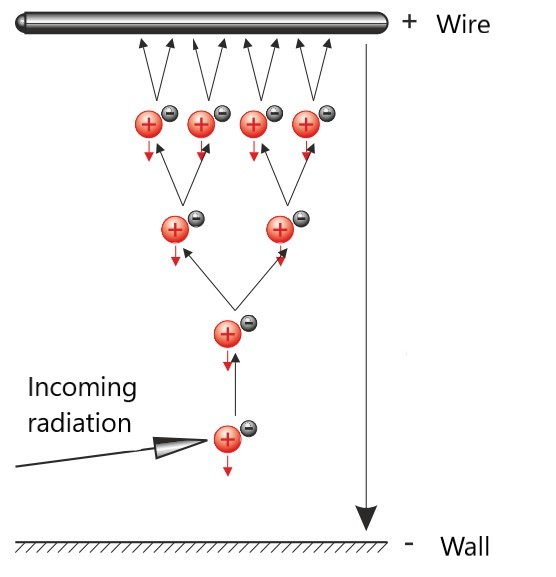
\includegraphics[width=.4\textwidth]{referenzen/scheme_avalanche.jpg}
    \caption{A single ionising event releases an avalanche of free electrons. These - fast enough accelerated toward the anode - form a pulse that can be further processed \cite{Eichler.2016}.}
    \label{fig:avalanche_discharge}
\end{figure}
To prevent the \(e^-\) to recombine before they reach the anode the accelerating voltage needs to be high enough. On the
other hand a voltage too high leads to spontanious self discharge of the inert gas. A rapid rise of counts can be observed
covering the actual ionisation events.
\begin{figure}[h]
    \centering
    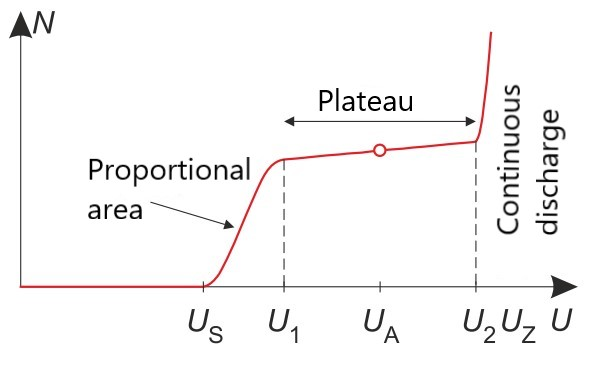
\includegraphics[width=.5\textwidth]{referenzen/gmt_plot.jpg}
    \caption[Characteristical curve of a GMT]{The characteristical curve of a GM-Tube. At a onset-voltage \(U_S\) the count rate is rapidly rising (plateau area). A certain voltage-range 
    is considered the working area (plateau). Further increase of the acceleration voltage leads to a second steep rise of counts (continuous discharge) \cite{Eichler.2016}.}
\end{figure}
%
%
While the preceding avalanche is not yet expired a new event will produce no pulses, hence, no counts can be measured.
This dead time is usually within the range of \(\SI{10^{-4}}{s}\). Still, the sensitivity of the GMT does not instantaniously
recover to full potential. Instead, for another period of time ongoing pules will gradually rise in magnitude until reaching
there original (maximum) level. In consequence some pulses may be too small for the downstream amplifying electronics to
trigger ultimately leading to undesired false-negatives i.e. too low count rate in a highly radiating environment.\par
%
%
\section{Stochastic Principles}
Since radioactive decay is a stochastic process, some usefull mathmatic principles need to be discussed.
\subsection{Binomial Distribution}
\begin{quote}
    A random experiment with only \textit{two mutually exclusive} results is called \textit{Bernoulli-experiment}\cite{Papula.MatheFormelsammlung.2017}
\end{quote}
Given an event has only two possible outcomes - \(A\) or \(\bar{A}\) - with the individual propabilities \(p(A) = 1 - p(\bar{A})\)
one can express the propability \(P\) for \(k\) successive events \(A\) within \(i\) repetitions as follows:
\begin{equation}
    P(k) = \binom{i}{k} \cdot p(A)^k \cdot p(\bar{A})^{i-k} \qquad \left( x \in \mathbb{N}_0 \right)
    \label{eq:binomWkt}
\end{equation}
Accordingly, the propability for \(k \leq x\) outcomes is expressed as
\begin{equation}
    P(k \leq x) = \sum_{k \leq x} \binom{i}{k}p(A)^k \cdot (1-p(A))^{i-k}
    \label{eq:binomVerteilung}
\end{equation}
and is called the distribution function.
In other words: summing up all individual propabilities \( P(x_j) \) gives the overall propability \( P \) to
encounter \textit{any} event out of the set of interest.
%
\subsection{\textsc{Poisson}-Distribution}
%
To reduce computational effort for large numbers of occurences \( x \) the \textsc{Poisson}-Distribution is often used.
Assuming an expected amount of \( \lambda \) occurences are expected to take place during a fixed time frame and assumed
further that each occurence is time independend and independent from each other one can calculate the possibility \( P \)
for any amount of occurences by
\begin{equation}
    P(k) = \frac{\lambda}{x!} \cdot e^{ -\lambda } \qquad \left( x \in \mathbb{N}_0 \right)
    \label[]{eq:poissonWkt}
\end{equation}
Again, \( x \) is the number of occurences of interest, \( \lambda \) the expected number of occurences.\par
Since the \textsc{Poisson}-Distribution is defined for all \( x \in \mathbb{N}_0 \) the sum of all single propabilities
\( P(x) \) equals 1. Thus, to get the propability to observe any amount of occurences during that time frame one can simply sum up
all individual propability as follows
%
\begin{equation}
    P(k \leq x) = e^{ -\lambda } \cdot \sum_{ k \leq x } \frac{\lambda^k}{k!}
    \label[]{eq:poissonVerteilung}
\end{equation}
%
\subsection{\textsc{Gauss}ian-Distribution}
%
Beeing interested in the propability of a distinct value \( x \) out of a continuous spectrum of values \( k \) with the
expected value \( \lambda \) and the standard deviation \( \sigma \) the \textsc{Gauss}ian- or Normal-Distribution gives
the propability for the occurence of a value \( x \) by
%
\begin{equation}
    P(k) = \frac{1}{\sqrt{2\pi}\sigma} \cdot e^{ - \frac{1}{2} \left( \frac{x - \mu}{\sigma} \right)^2 } \qquad \left( x \in \mathbb{R} \right)
    \label[]{gaussWkt}
\end{equation}
%
with the distribution function accordingly
\begin{equation}
    P(k \leq x) = \frac{1}{\sqrt{2\pi}\sigma} \cdot \int_{ -\infty }^x e^{ -\frac{1}{2} \left( \frac{x - \mu}{\sigma} \right)^2 } dx
\end{equation}
\chapter{Set-up of experiment}
%
Some equipment and materials are needed to perform the experiments. These are shown in the fig. \ref{fig:setup} and listed again below.
%
\begin{figure}[H]
	\begin{center}
		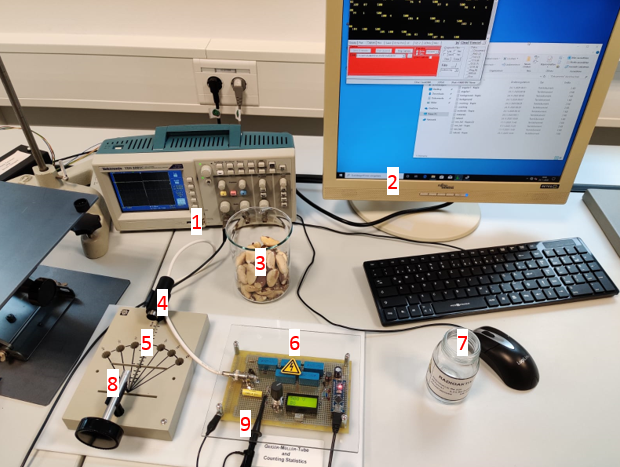
\includegraphics[width=.9\textwidth]{aufbau/setup.PNG} % changed to local path
		\caption{Equipment and material required for the experiments.}  
		\label{fig:setup} 
	\end{center}
\end{figure}
%
\begin{enumerate}
	\item Oscilloscope
	\item Computer with the software RealTerm
	\item Beaker with Brazil nuts
	\item Geiger-Müller tube
	\item Mounting plate
	\item Circuit board
	\item Protective container
	\item Radioactive source ($^{226}$Ra, 3.3 kBq)
	\item Oscilloscope probe with ground clip
\end{enumerate}
%
A better view of the circuit board will give fig. \ref{fig:circuit_board}. Again, the components are listed below.
%
\begin{figure}[H]
	\begin{center}
		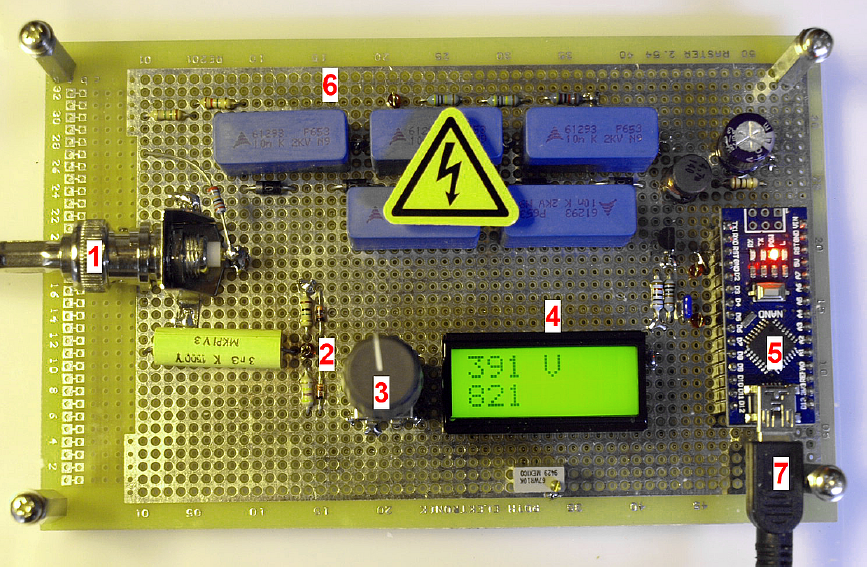
\includegraphics[width=.9\textwidth]{aufbau/circuit_board.png}
		\caption{Circuit board in greater detail. (Source: A. Dörr, Geiger-Müller Tube and Counting Statistics, page 5)}  
		\label{fig:circuit_board} 
	\end{center}
\end{figure}
%
\begin{enumerate}
	\item BNC connector
	\item Testpoint
	\item Potentiometer
	\item LCD
	\item Arduino nano
	\item Boost converter
	\item USB port
\end{enumerate}
%
To begin with the experiments, the computer is started first. When the computer is ready, the program RealTerm is being started. The following settings are made:
\begin{itemize}
	\item In the \texttt{Port} tab, 9600 is selected for \texttt{Baud}.
	\item The microcontroller is connected with the computer and the assigned COM number is selected under \texttt{Port}.
	\item On the \texttt{Display} tab, \texttt{Ascii} and \texttt{new Line mode} are checked, \texttt{Direct capture} is un-checked.
\end{itemize}
%
The data is now continuously sent by the microcontroller. The data is displayed on the screen. A text file is created in which the data is written and saved. Three columns are displayed. The first column contains the number of the measurement, the second the counts per 10 s and the third the present voltage $U_{GMT}$.\\
Now the oscilloscope is switched on. The probe tip is connected to the test point. The ground clip is attached to the housing of the circuit board. The display is adjusted so that a single radioactive event fills the screen when the trigger is set correctly.\\
Now the setup is completed and the experiments can be started.
\input{chapters/4_durchführung}
\chapter{Evaluation}
%
\section{GMT characteristics}
%
\subsection{Characteristic values of the oscilloscope}
%
The signal of the GMT can be seen on the oscilloscope screen (s. fig.1-5). fig.1 shows us the zero level \(U_{0}\) and
the amplitude \(\hat{U}\):
%
\begin{align}
    U_{0}   &=  \SI{24}{mV} \pm \SI{40}{mV} \\
    \hat{U} &=  \SI{1,56}{V} \pm \SI{0,04}{V}
\end{align}
%
Further there can be read off the fall time \(t_{f}\) (fig.2), rise time \(t_{r}\) (fig.3), the pulse width \(t_{p}\)
(fig.4) and recovery time \(t_{re}\) (fig.5):
\begin{align}
    t_{f}   &=  \SI{56}{\micro s} \pm \SI{20}{\micro s} \\
    t_{r}   &=  \SI{228}{\micro s} \pm \SI{20}{\micro s} \\
    t_{p}   &=  \SI{108}{\micro s} \pm \SI{20}{\micro s} \\
    t_{re}  &=  \SI{288}{\micro s} \pm \SI{20}{\micro s}
\end{align}
-fig.1-\\
-fig.2-\\
-fig.3-\\
-fig.4-\\
-fig.5-
%
\subsection{Characteristic curve of the GMT}
%
After determining the starting voltage \(U_{start}\) to \(U_{start}=\SI{328}{V}\), the characteristic curve has been
recorded by measuring the count rate over 100 seconds for each step-by-step-increased voltage. The calculated mean value
of the count rate has been plotted versus the mean voltage by SciDAVis:\par
-fig.6-\par
The relative slope in the plateau area is determined to \(m=(3,2 \pm 2,8) \frac{\%}{\SI{100}{V}}\) by SciDAVis.\par
The optimum working voltage \(U_{opt}\) is determined to \(U_{opt}=\SI{500}{V}\), since the maximum possible adjustable
voltage of \(U_{GMT}=\SI{600}{V}\) is still in the plateau area, which starts at \(U_{GMT}=\SI{340}{V}\).
%
\section{Angular dependency of the count rate}
To examine the angular dependency of the count rate the angle of the tube has been varied from \SI[]{-45}[]{\degree} to
\SI[]{+45}[]{\degree} in \SI[]{15}[]{\degree} steps. After measuring the count rate at the optimum working voltage of
\(U_{opt}=\SI{500}{V}\) and calculating the mean value of the 12 count rates of each angle, the count rate was output
versus angle by SciDAVis:\par
-fig.7-\par
%
\section{Absorption characteristics of materials}
%
For investigating the absorption characteristics of materials the count rate has been measured 12 times at
\(U_{opt}=\SI{500}{V}\) for different materials (\(\text{thickness}=\SI{2}{mm}\)) in front of the tube:
%
\begin{align}
    &\text{no absorbing material: }  &&n = \SI{221}{cps} \pm \SI{11}{cps}\\
    &\text{Aluminum (Al): }          &&n = \SI{10}{cps} \pm \SI{4}{cps}\\
    &\text{Lead (Pb): }              &&n = \SI{7}{cps} \pm \SI{2}{cps}\\
    &\text{Tin (Sn): }               &&n = \SI{6}{cps} \pm \SI{2}{cps}\\
    &\text{Acrylic glass: }          &&n = \SI{26}{cps} \pm \SI{5}{cps}\\
    &\text{Cardboard: }              &&n = \SI{104}{cps} \pm \SI{8}{cps}
\end{align}
%
The explanation for the different absorption of the different materials is the mass attenuation coefficient of the
different materials. The mass attenuation coefficient is dependent on the material density \(\rho\) and the attenuation
coefficient \( \mu \). Since the attenuation coefficient depends on the atomic number, the size of the atom does
matter. The reason why there is happening an attenuation is because of the \(\alpha\)-, \(\beta\)- and \(\gamma\)-rays are
interacting with the material atoms. While the \(\alpha\)- and \(\beta\)-rays have a strong interaction with the material,
\(\gamma\)-rays have better penetration due to less likeliness to interact. The smaller the half-value layer of a
material the weaker the penetration. With lead (\isotope[82]{Pb}) and Tin (\isotope[50]{Sn}) and presumably Aluminum
(\isotope[13]{Al}) as well almost all rays are absorbed (dependent on the ray energy). Acrylic glass can probably be
traversed by the \(\gamma\)-rays. Due to there size already a thin sheet of cardboard is sufficient to absorbed
\(\alpha\)-ray particles almost entirely.
%
\section{Counting statistics}
%
For examining the statistics, 90 measurements were taken at a distance of \( \SI{1}{cm} \) and a voltage of
\( U_{opt}=\SI{500}{V} \). The following values for mean \( \bar{n} \), variance \( \sigma^{2} \) and standard deviation
\( \sigma \) were obtained:
%
\begin{align}
    \bar{n}     &=  \SI{4327}{cps} \\
    \sigma^{2}  &=  \SI{4168}{(cps)^{2}} \\
    \sigma      &=  \SI{65}{cps}
\end{align}
The measurement series results a scatter plot in SciDAVis:\par
-fig.8-\par
A histogram made with SciDAVis shows the distribution of the measures:\par
-fig.9-\par
With radioactive decay it cannot be said which atom will decay when. Since it is a statistical process, the histogram
can be described with a Poisson-distribution.
%
\section{Background radiation}
%
To investigate the background radiation the count rate was measured 90 times with no radiation source at a voltage of
\( U_{opt}=\SI{500}{V} \). The measurement stats are:
%
\begin{align}
    \bar{n}     &=  \SI{3}{cps} \\
    \sigma^{2}  &=  \SI{20}{(cps)^{2}} \\
    \sigma      &=  \SI{4}{cps}
\end{align}
The measurement number was plotted versus the count rate by SciDAVis:\par
-fig.10-\par
The associated distribution histogram was drawn by SciDAVis:\par
-fig.11-\par
This histogram can also be described by a Poisson-distribution for the same reason as histogram of the counting
statistics.
%
\section{Natural radioactivity}
%
The radioactivity of a package Brazil nuts should have been determined by measuring the count rate. For that the GMT was
put in a beaker filled with Brazil nuts for 900 seconds at \( U_{opt}=\SI{500}{V} \).\par
The mean value of \( \bar{n}=\SI{3}{cps} \) indicates that the radioactivity of the Brazil nuts is very weak because it
has the same mean value as the background radiation. However, this does not have to mean that the Brazil nuts do not emit
any radiation. Because the tube was very close to the nuts, the background radiation could not pass directly through the
nuts, which implies that the rest of the radiation must have come from the Brazil nuts.\par
-fig.12-
\chapter{Conclusion}
%
In a closing statement, the experiment is applicable to investigate the properties of a \textsc{Geiger-Mueller} tube and
clearly shows effects of radioactive decay. The oscilloscope shows the GMTs signal with its characteristic patterns
values as well as the recorded curves beeing very similar to the expected ones.\par
Unfortunately, the maximum adjustable voltage was only \( 600 V \). Therefore, the measurement ended somewhere in the
plateau area. The angular dependency of the count rate is plausible, as fewer particles arrive at an effective spatial
angle. The different absorption materials show that different material properties have a rather huge impact the rays passing
through. While some could drop the count rate to a degree comparable to the blank measurement discribed in \cref{sec:backgroundRadiation}
other seemingly had no impact at all. The raw measurement illustrates the statistical decay processes as well as the
functionality of the GMT.\par
Even though it was already common sense, measuring and visualizing the omnipresent background radiation as well as making
radioactivity of digestibles visible was a fascinating excercise. Plans are rising to give building a cloud chamber another
go.\par\medskip
While we assume it to be rather simple, yet we missed an introduction to the code used on the \micro-controller.
%-------------------
\newpage
\listoffigures 
\listoftables
\addchap{List of Symbols}
\begin{table}[h]
    \begin{tabular}{@{}ll@{}}%
        \( A \) & Distinct event\\
        \( d \) & Distance\\
        \( i \) & Repetitions\\
        \( k \) & Amount of events\\
        \( m \) & Mass\\
        \( N \) & Non-decayed nuclei\\
        \( n \) & Amount of counts\\
        \( \bar{n} \) & Mean counts\\
        \( T_{\nicefrac{1}{2}} \) & Half-life\\
        \( t \) & Time\\
        \( t_f \) & Fall time\\
        \( t_p \) & Pulse width\\
        \( t_r \) & Rise time\\
        \( t_{ re } \) & Recovery time\\
        \( P \) & Possibility for one or more events\\
        \( p \) & Single-event possibility\\
        \( \hat{U} \) & Peak voltage\\
        \( U_0 \) & Base line voltage\\
        \( U_{ GMT } \) & Actual voltage\\
        \( U_{ opt } \) & Optimum voltage of operation\\
        \( U_{ Start } \) & Voltage at which counts begin to get registered\\
        \( x \) & Occurence of interest\\
        & \\
        \( \lambda \) & Expected value\\
        \( \sigma \) & Standard deviation\\
        \( \sigma^2 \) & Empirical variance\\
        \( \tau \) & Mean lifespan\\
    \end{tabular}
    \label{tab:glossar}
\end{table}
%\printnomenclature
\appendix
\chapter{Appendix}

\begin{figure}[!ht]
    \centering
    \subfloat[Amplitude \(\hat{U}\)\label{subfig:pulsAmplitude}]{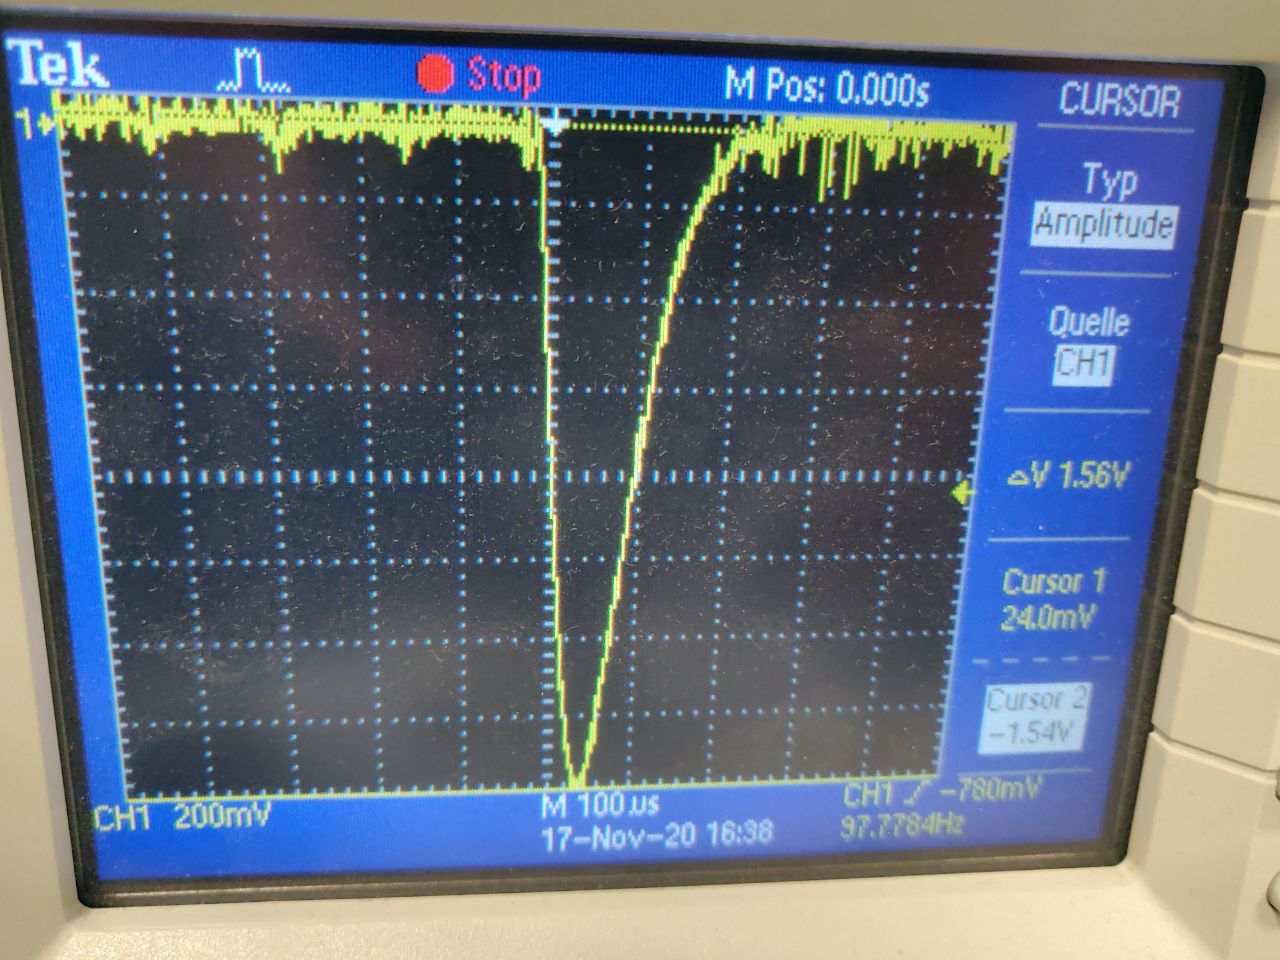
\includegraphics[width=0.45\textwidth]{messdaten/Fig.1_pulsAmplitude.jpg}}
    \hspace{.05\textwidth}
    \subfloat[Fall Time \(t_{f}\)\label{subfig:fallTime}]{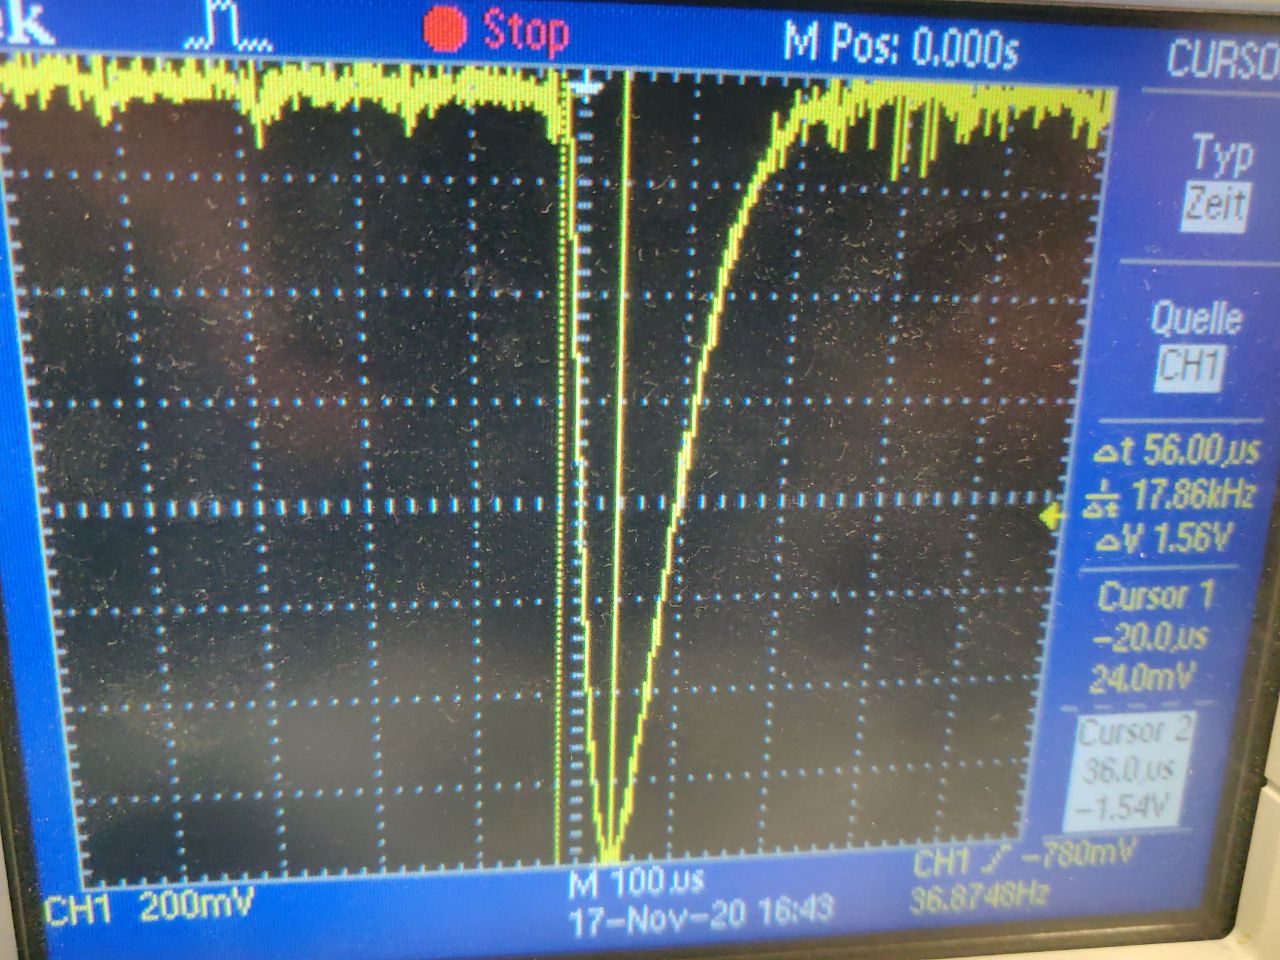
\includegraphics[width=0.45\textwidth]{messdaten/Fig.2_fallTime.jpg}}
    \hspace{.2\textwidth}
    \subfloat[Rise Time \(t_{r}\)\label{subfig:riseTime}]{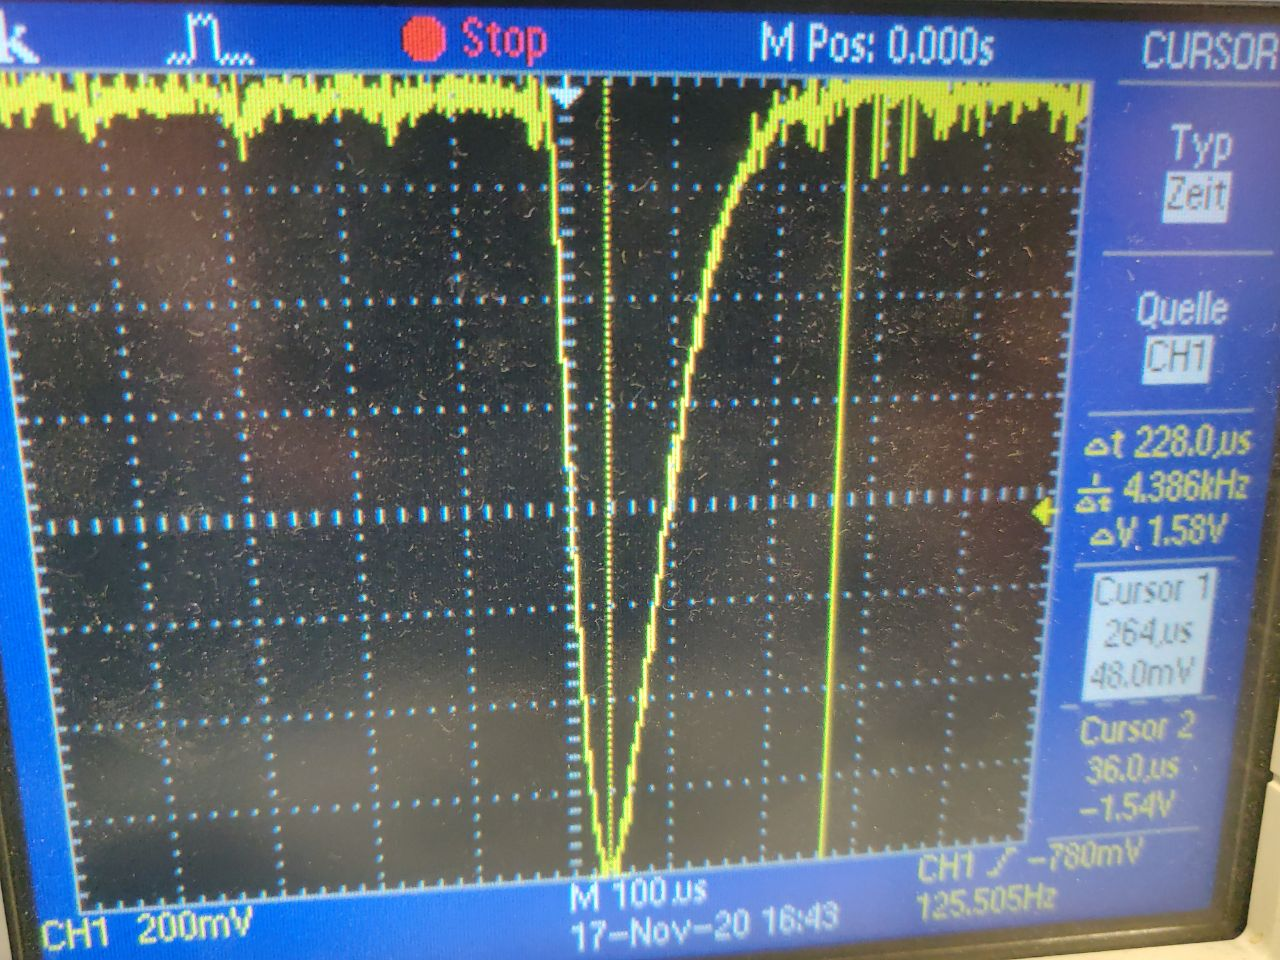
\includegraphics[width=0.45\textwidth]{messdaten/Fig.3_riseTime.jpg}}
    \hspace{.05\textwidth}
    \subfloat[Pulse Width \(t_p\)\label{subfig:pulseWidth}]{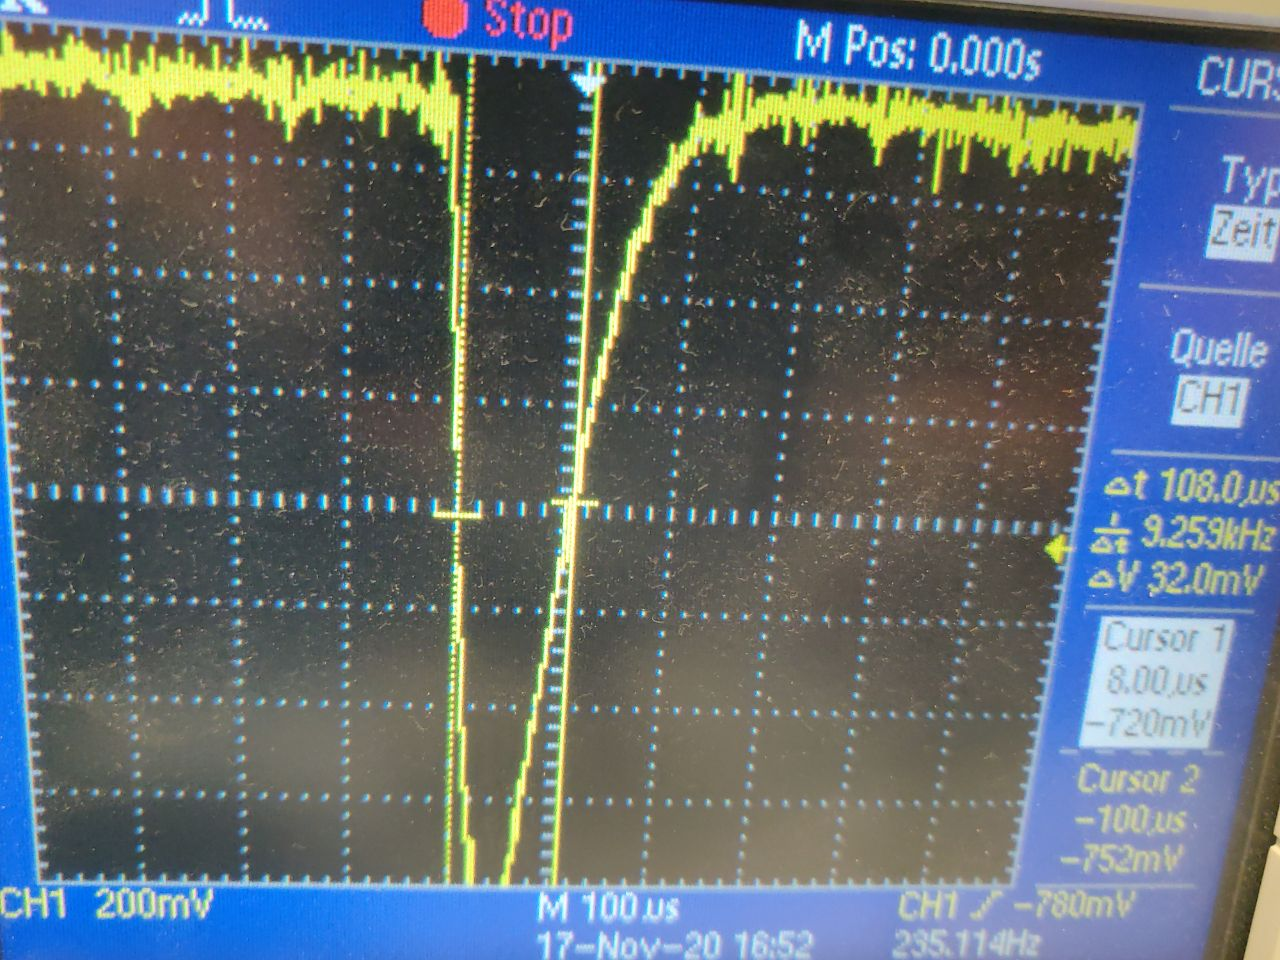
\includegraphics[width=0.45\textwidth]{messdaten/Fig.4_pulseWidth.jpg}}
    \hspace{.2\textwidth}
    \subfloat[Recovery Time \(t_{r}\)\label{subfig:recoveryTime}]{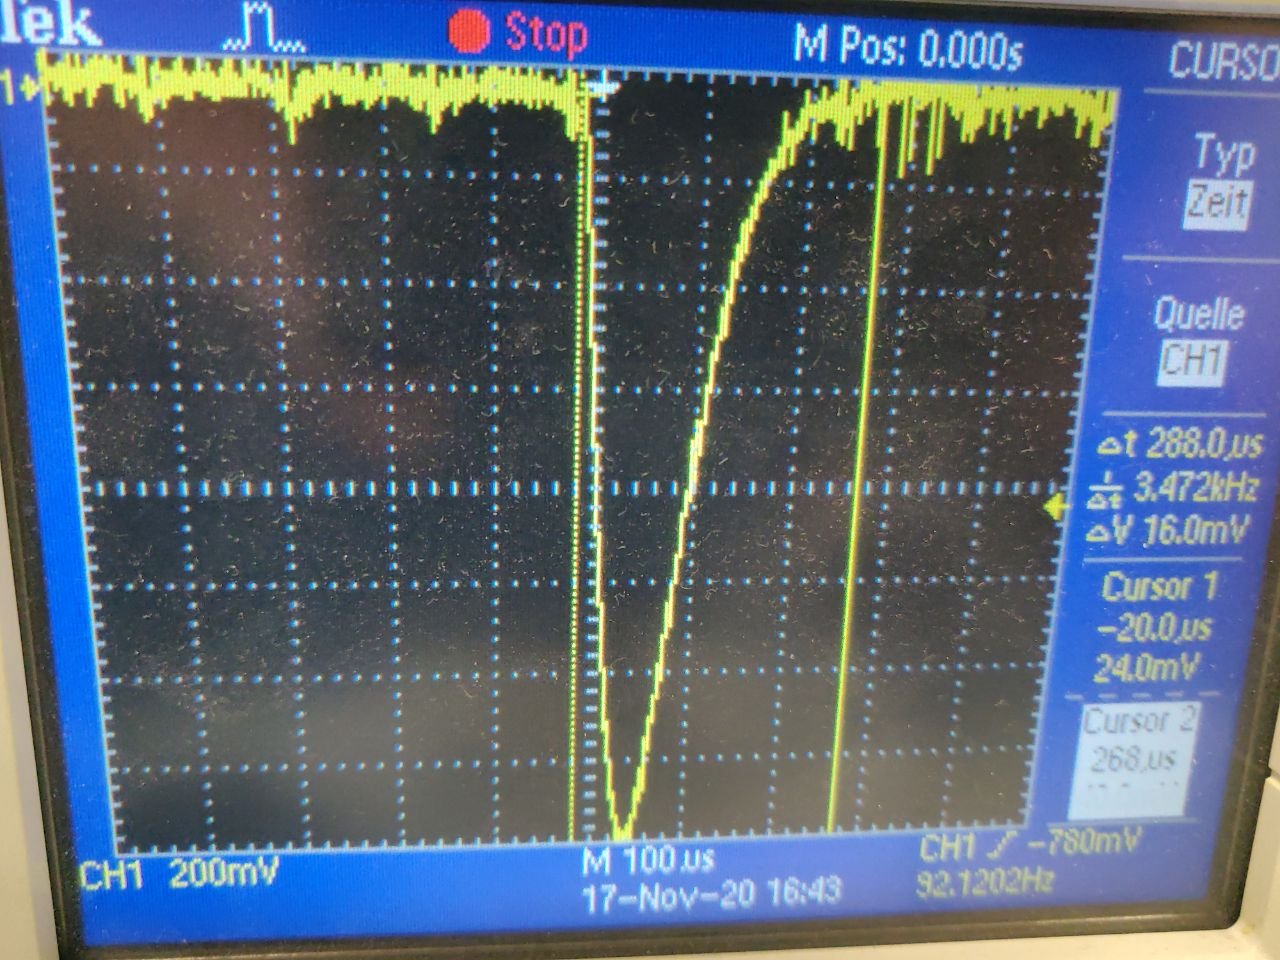
\includegraphics[width=0.45\textwidth]{messdaten/Fig.5_recoveryTime.jpg}}
    \caption[Oszillograms]{During the course of the experiment captured oscillograms.}
 \end{figure}
 %
 \newpage
 %
%\bibliography{Z:/Dokumente/HSRM/LaTex_Quellen/HSRM_Quellen/quellen}
\printbibliography
%\bibliographystyle{plaindin}
%==========================================
\end{document}